\title{}
\subtitle{Extending foundational concepts with our coal-fired power plant example}
\author{
	\begin{itemize}
		\item Why textbook examples fail mixtures
		\item Inverse probability weighting and G-computation
		\item Wrap-up
	\end{itemize}
}
\date{}
\begin{frame}
	\titlepage
\end{frame}


%%%%%%%%%%%%%%%%
\begin{frame}[t]
  \frametitle{Textbook examples fail us for mixtures}
Our textbook examples have only included on single binary exposure $A$. 

\bigskip
But mixtures have continuous, and potentially highly exposures, so we'll almost always have sparsity where certain ranges of exposure just are not observed for different covariate/exposure strata.

\bigskip
And a mixture of multiple exposures (Arsenic, Beryllium, Cadmium) means we can't rely (without modification) on the wealth of methods for single exposures. 

%\bigskip
%Mixtures also often bring up issues of environmental justice (e.g. historical exposure inequity due to racism) 

\end{frame}



\begin{frame}[t]
We'll investigate these issues without resorting to (too much) notation. Recall our (simulated) example 
{\footnotesize
	  \begin{tikzpicture}[>=latex, line join=bevel, very thick]
	     %
             \node[](coal){\begin{tabular}{c}Proximity to \\ coal fired plant\end{tabular}};
             \node[above right=of coal, shift={(0,-1)}](a){Arsenic $(A)$};
             \node[right=of coal](b){Beryllium $(B)$};
             \node[below right=of coal, shift={(0,1)}](c){Cadmium $(C)$};
             \node[ right=of b] (y) {\begin{tabular}{c}Mental development\\ index $(Y)$\end{tabular}};
             \node[above =of a] (w1) {\begin{tabular}{c}\\Black race $(W2)$\end{tabular}};
             \node[above =of w1, shift={(0,-1)}] (w2) {\begin{tabular}{c}Urbanicity $(W1)$\end{tabular}};
             %
             \path[-latex] (coal) edge[] (a);  
             \path[-latex] (coal) edge[] (b);  
             \path[-latex] (coal) edge[] (c);  
             \path[-latex] (a) edge[] (y);  
             \path[-latex] (b) edge[] (y);  
             \path[-latex] (c) edge[] (y);  
             \path[-latex] (a) edge[] (y);  
             \path[latex-latex] (w1) edge[style=dashed] (y);  
             \path[-latex] (w1) edge[] (coal);  
             \path[-latex] (w2) edge[bend right] (coal);  
             \path[latex-latex] (w2) edge[style=dashed, bend left] (y);  
          \end{tikzpicture} 
}
\end{frame}

\begin{frame}[t]{Basics of the data}
    \begin{columns}
    \begin{column}[t]{.6\textwidth}
    The first 5 observations
	  % Table generated by Excel2LaTeX from sheet 'Sheet1'
\begin{tabular}{rrrrrr}\hline
\multicolumn{1}{l}{urbanicity} & \multicolumn{1}{l}{black} & \multicolumn{1}{l}{as} & \multicolumn{1}{l}{be} & \multicolumn{1}{l}{cd} & \multicolumn{1}{l}{mdi} \\\hline
1     & 0     & 0.814 & 0.931 & 1.64  & 82.5 \\
0     & 0     & 0.243 & 0.354 & 0.243 & 93.9 \\
1     & 0     & 0.404 & 0.406 & 0.665 & 123 \\
0     & 1     & 0.366 & 0.241 & 0.218 & 115 \\
1     & 0     & 0.245 & 0.347 & 0.335 & 110 \\\hline
\end{tabular}%
    \end{column}
    \begin{column}[t]{.4\textwidth}
    Pearson correlation matrix
	  % Table generated by Excel2LaTeX from sheet 'Sheet2'
\begin{tabular}{l|r|r|r|}
\multicolumn{1}{r}{} & \multicolumn{1}{l}{as} & \multicolumn{1}{l}{be} & \multicolumn{1}{l}{cd} \bigstrut[b]\\
\cline{2-4}as    & 1     &   &  \bigstrut\\
\cline{2-4}be    & 0.86  & 1     &  \bigstrut\\
\cline{2-4}cd    & 0.76  & 0.68  & 1 \bigstrut\\
\cline{2-4}\end{tabular}%
    
    \end{column}
  \end{columns}
  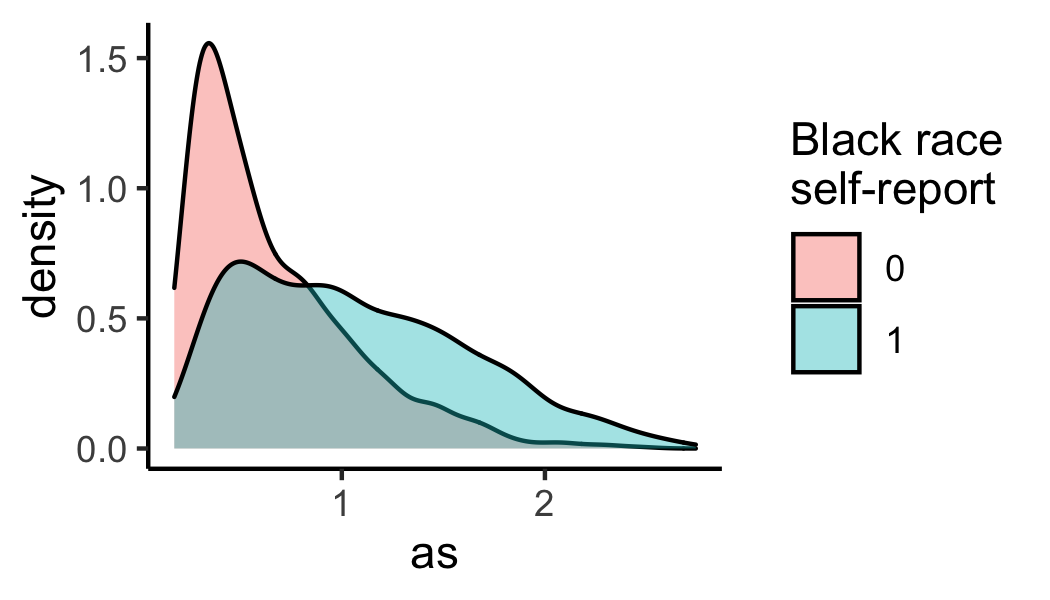
\includegraphics[height=.15\textwidth]{../analyses/output/as_dens.png}%
  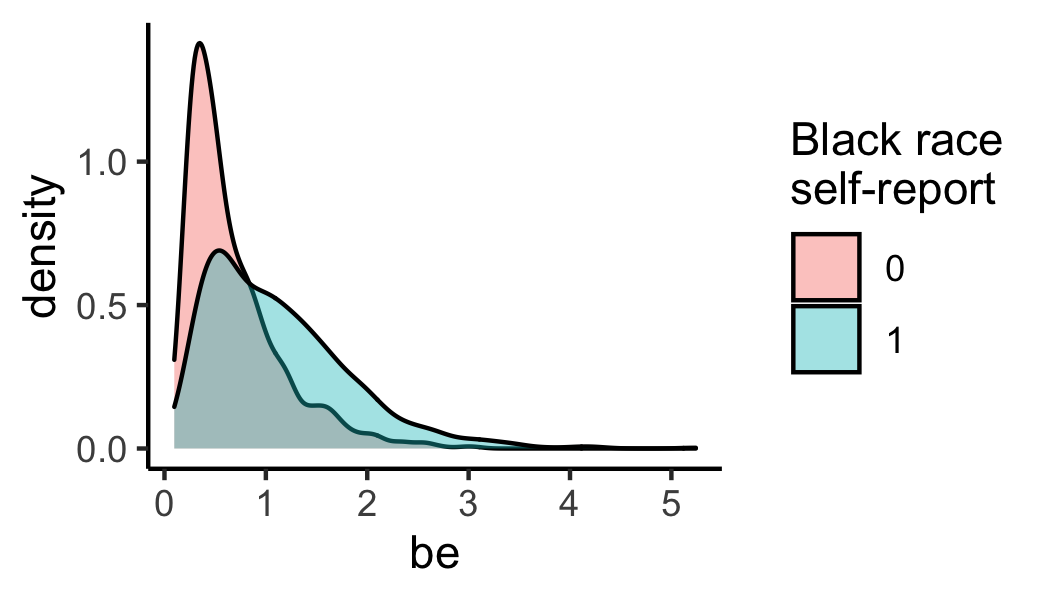
\includegraphics[height=.15\textwidth]{../analyses/output/be_dens.png}%
  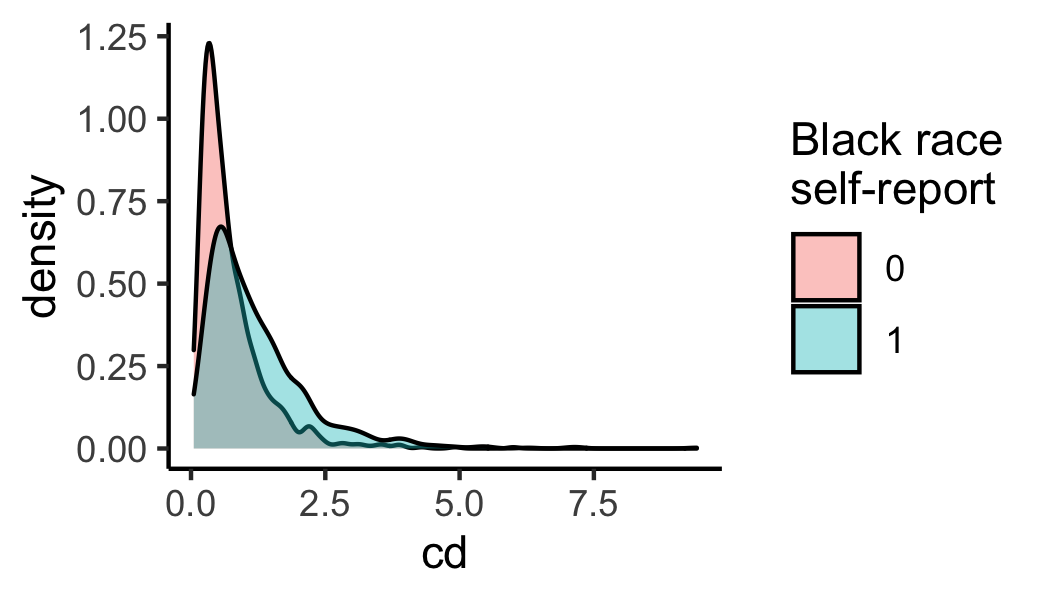
\includegraphics[height=.15\textwidth]{../analyses/output/cd_dens.png}%
  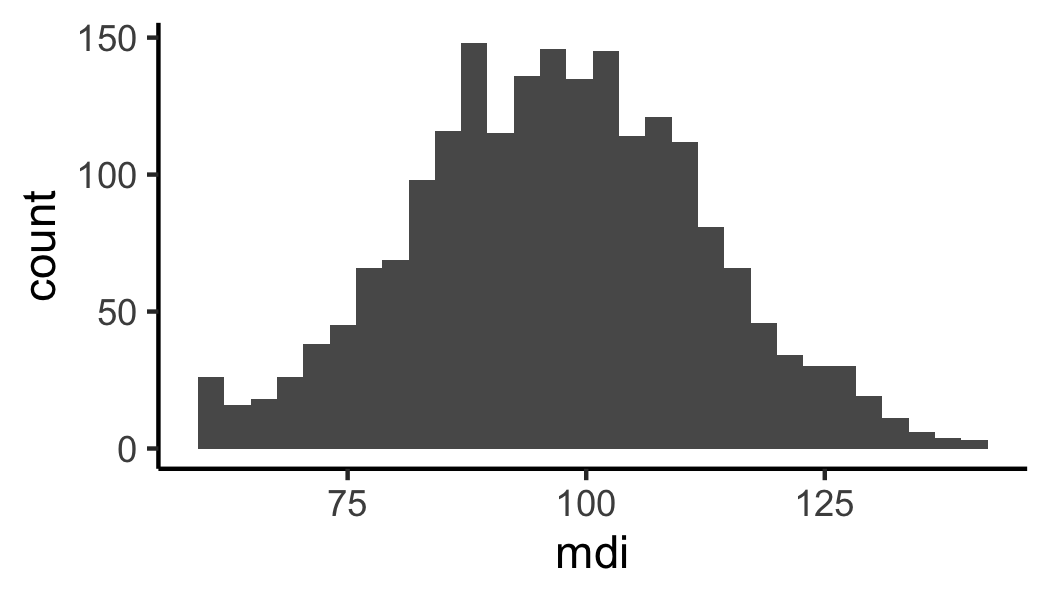
\includegraphics[height=.15\textwidth]{../analyses/output/mdi_dens.png}
\end{frame}


\begin{frame}[t]{Textbook examples and continuous exposures}
Under our DAG, for a single exposure (say arsenic), the "minimal causal unit" that we need is:
$$
E(MDI | A=a, B=b, C=c, Confounders)
$$
Roughly, to identify a causal effect of increasing arsenic by 1 unit (e.g. an independent causal dose response), we would need to observe, roughly, that at all values of the other exposures and confounders, we see some variation in arsenic of about 1 unit.\footnote{Sort of, this is language for discrete variables, which is fuzzy to apply here but to be more exact requires measure theory :(}
\end{frame}



\begin{frame}[t]{Textbook examples and continuous exposures}
 
   \begin{columns}
    \begin{column}[c]{.5\textwidth}
     \only<1>{Visually, we can see whether sparsity is an issue (it is, and we've known it for a long time)\footnotemark}
     \only<2>{
       Here we can see that a one unit change (1.5 $\rightarrow$ 2.5) in arsenic is possible and (informally) identified when Beryllium = 1.0 ug/m$^3$
       \bigskip
       
       "Identification" here just informally means that we have some data points on both the left and right sides of the red bar, where the MDI for those individuals would be used in estimating the causal contrast (very roughly speaking)
       
     }
     \only<3>{It may be possible (positivity) but it is not observed (sparsity) when Beryllium = 3.0 ug/m$^3$}
     \only<4>{This issue is well described and it seems hopeless that we'll be biased.}
     \only<5>{However, note that, a 1 unit change  (2.5 $\rightarrow$ 3.5) in arsenic is observed  when Beryllium = 3.0 ug/m$^3$}
     \only<6>{If we can assume that the rate of change (e.g. regression coefficient) of the outcome is modeled accurately within the range of the data, then the effect of  As = 1.5 $\rightarrow$ As = 2.5, is "parametrically" identified.
     \bigskip
     
     A statistical model allows us to share information to estimate valid causal effects where we have no data, \emph{provided the model is correct}. This is dangerous and difficult to diagnose, but (caveat emptor) it's possible.
     }
     \only<7>{The amount of extrapolation and reliance on assuming a correct model grows very quickly as we condition on more and more exposures/confounders, which is part of the \textbf{curse of dimensionality} }
    \end{column}
    \begin{column}[c]{.5\textwidth}
    \begin{figure}
		 \only<1>{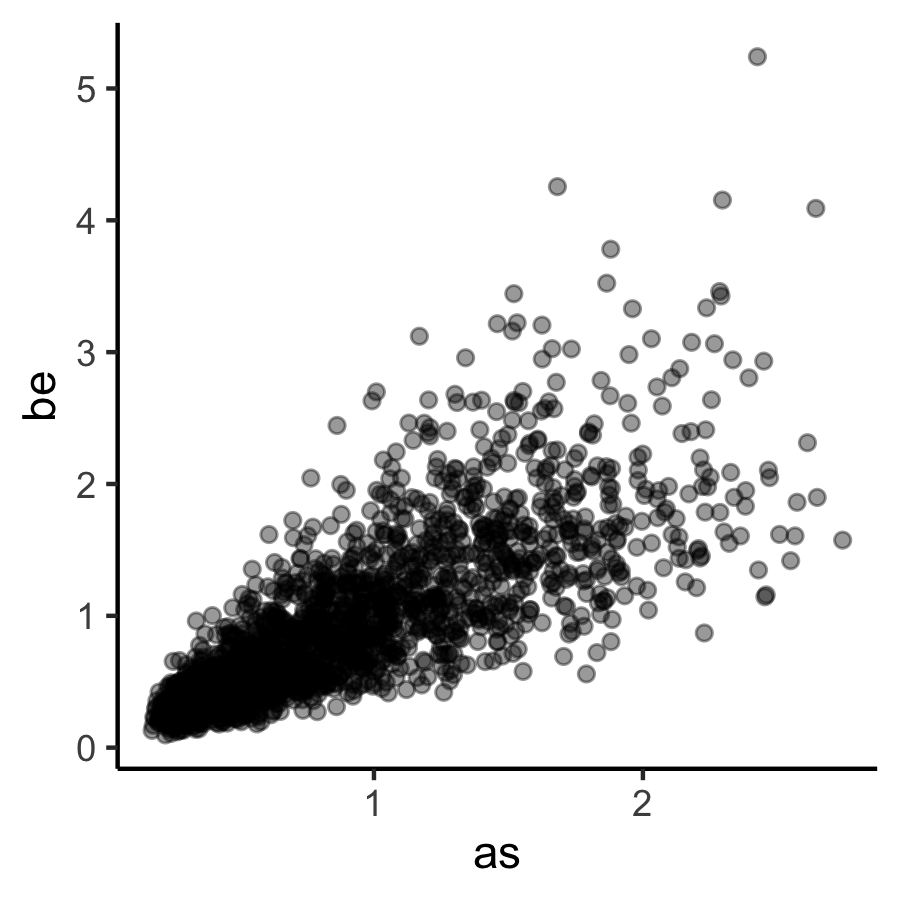
\includegraphics[height=.8\textheight]{../analyses/output/as_be_scatter.png}}%
		 \only<2>{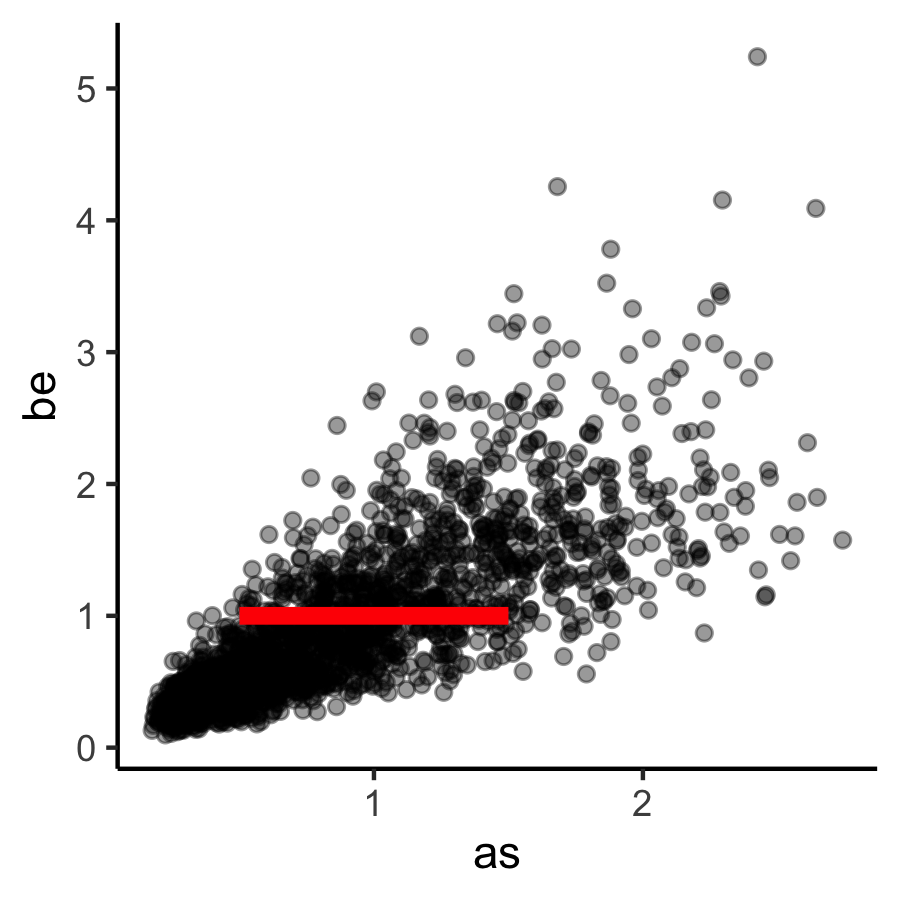
\includegraphics[height=.8\textheight]{../analyses/output/as_be_scatter_b1.png}}%
		 \only<3,4>{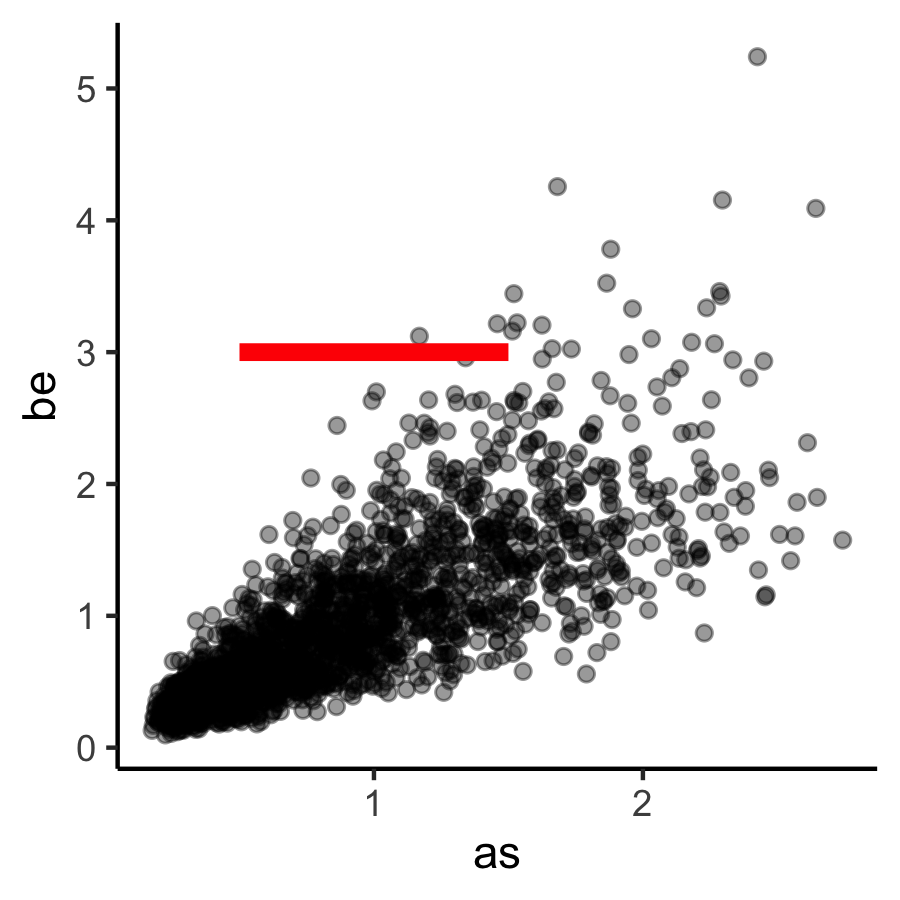
\includegraphics[height=.8\textheight]{../analyses/output/as_be_scatter_b2.png}}%
		 \only<5>{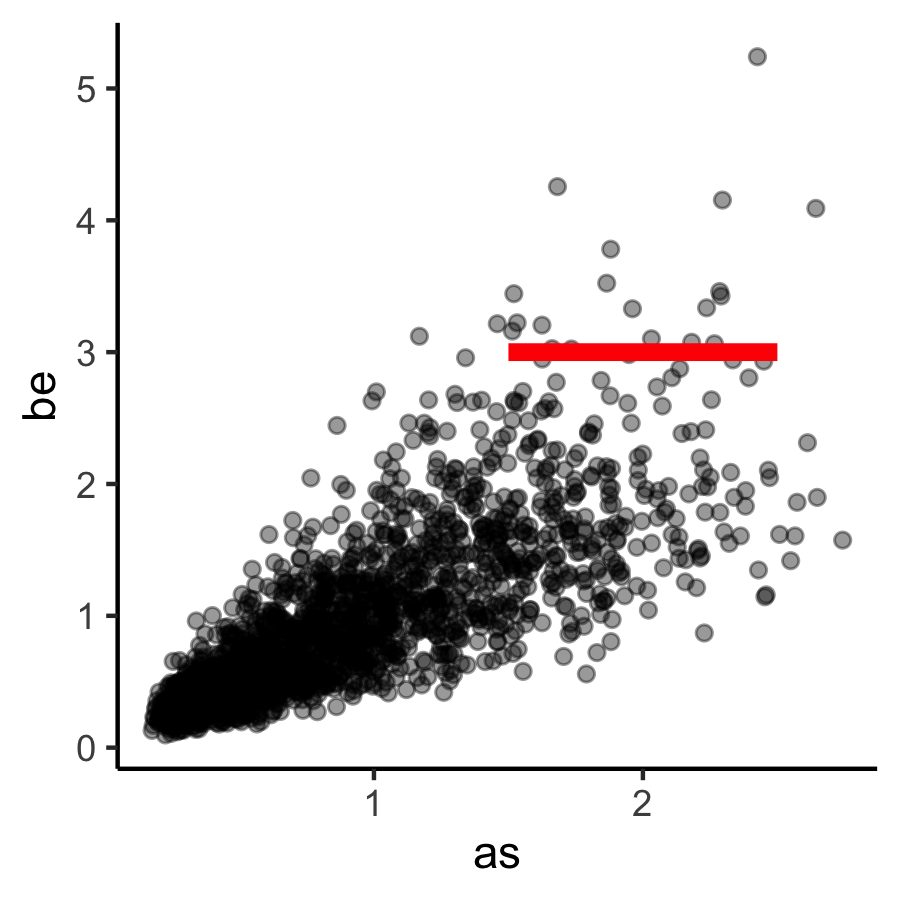
\includegraphics[height=.8\textheight]{../analyses/output/as_be_scatter_b3.png}}%
		 \only<6->{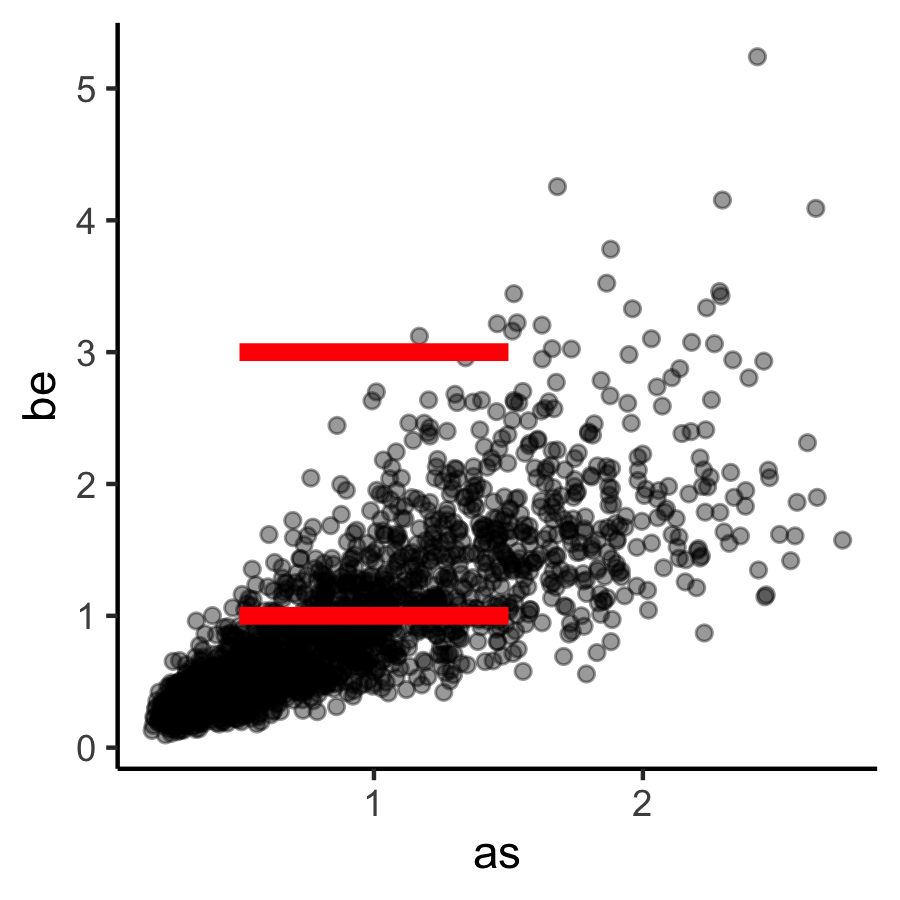
\includegraphics[height=.8\textheight]{../analyses/output/as_be_scatter_b4.png}}%
   \end{figure}
   \end{column}
  \end{columns}
 \only<1>{ \footnotetext{Snowden, et al. Framing air pollution epidemiology in terms of population interventions, with applications to multi-pollutant modeling. Epidemiology 26.2 (2015): 271.}}
\end{frame}

\begin{frame}[t]{Continuous exposures beyond textbook examples}
The curse of dimensionality is part of the \textbf{fundamental problem of mixtures}: correlation between components of a mixture means we should suspect co-pollutant confounding, but adjusting for that confounding in statistical models can lead to problems on its own. To address this information problem, causal inference in mixtures can potentially benefit from: 
\bigskip

    \begin{itemize}
      \item Dimension reduction (PCA, clustering, profile regression)
      \item Shrinkage, selection, Bayesian priors (LASSO, E-net, Bayesian regression/selection, other regularized machine learning)
      \item {\only<2>{\color{red}}Changing the question} (WQS, Bayesian kernel machine regression, quantile g-computation)
    \end{itemize}


\end{frame}


\begin{frame}[t]{Textbook examples and multiple exposures} 
  \begin{columns}
    \begin{column}[c]{.5\textwidth}
	    \only<1>{Textbook examples of causal inference rarely mention more than one exposure}
	    \only<2>{The fundamental problem of mixtures really describes problems with estimating the effect of one exposure, holding others constant: }
   	    \only<3>{Alternatively, consider the effect of two exposures, where the contrast is again roughly a comparison of the average outcomes at each end of the red line:  }
   	    \only<4>{Here we transform exposure so that "1 unit" of exposure is "1 quantile" (e.g. a quartile length)}
   	    \only<5->{This effect is occasionally discussed in the textbook examples as a "joint effect"
	    \bigskip
             
             see e.g. VanderWeele, T. J. (2009). On the distinction between interaction and effect modification. Epidemiology, 20(6), 863-871.}
    \end{column}
    \begin{column}[c]{.5\textwidth}
    		 \only<1>{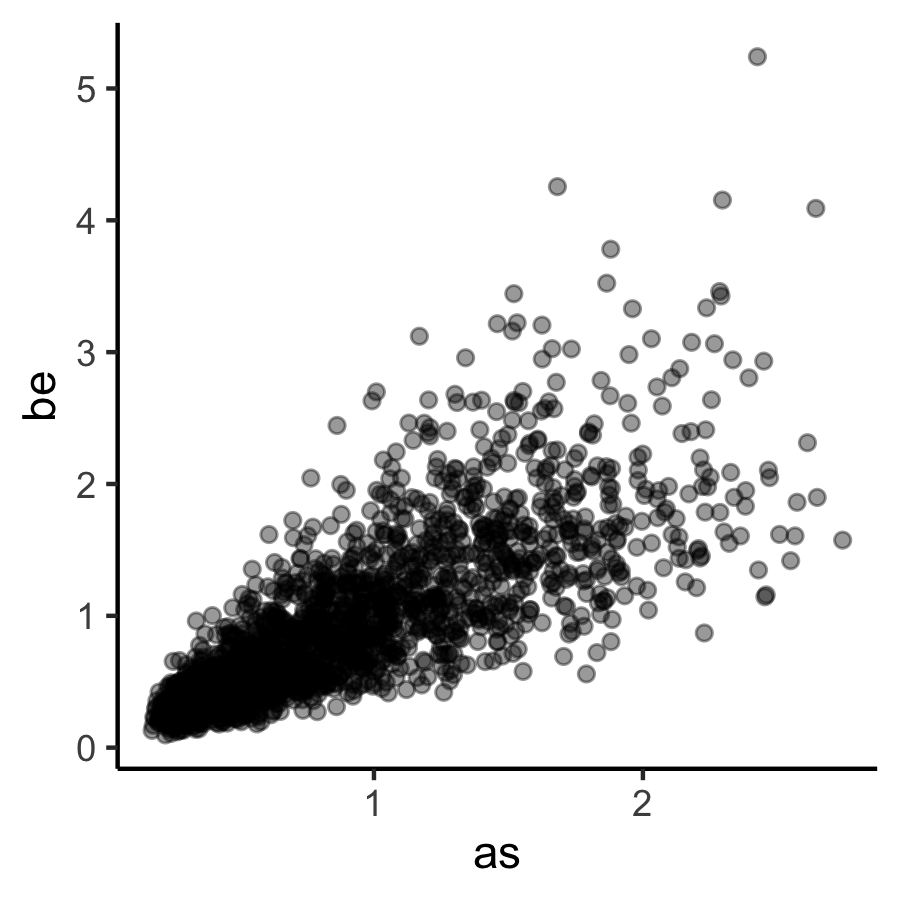
\includegraphics[height=.8\textheight]{../analyses/output/as_be_scatter.png}}%
    		 \only<2>{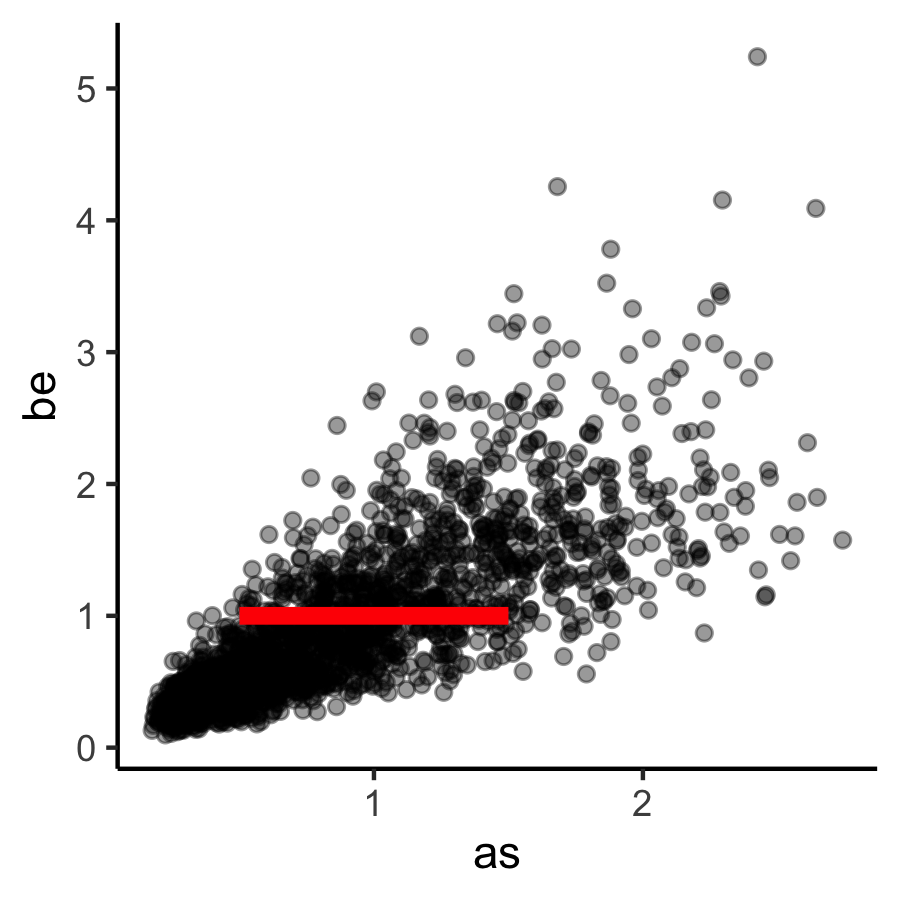
\includegraphics[height=.8\textheight]{../analyses/output/as_be_scatter_b1.png} $$E(y^{a+1}|b=1) - E(y^{a}|b=1)$$}%
    		 \only<3>{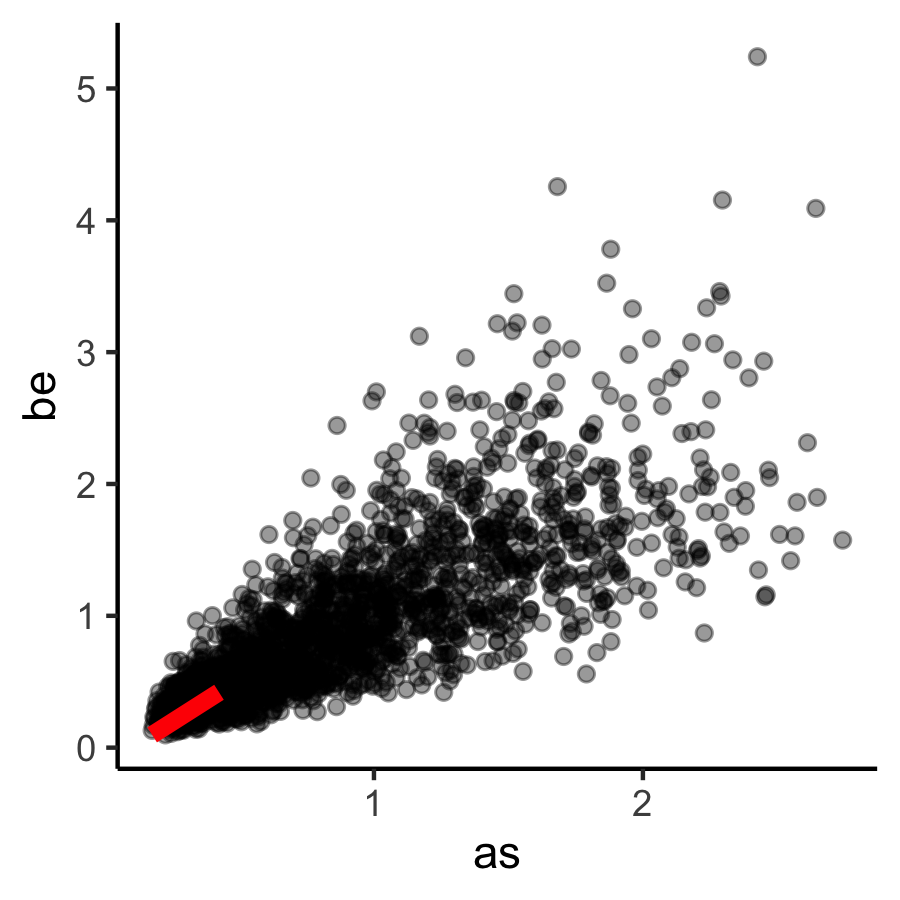
\includegraphics[height=.8\textheight]{../analyses/output/as_be_scatter_j1.png} $$E(y^{a+1, b+1}) - E(y^{a,b})$$}%
    		 \only<4>{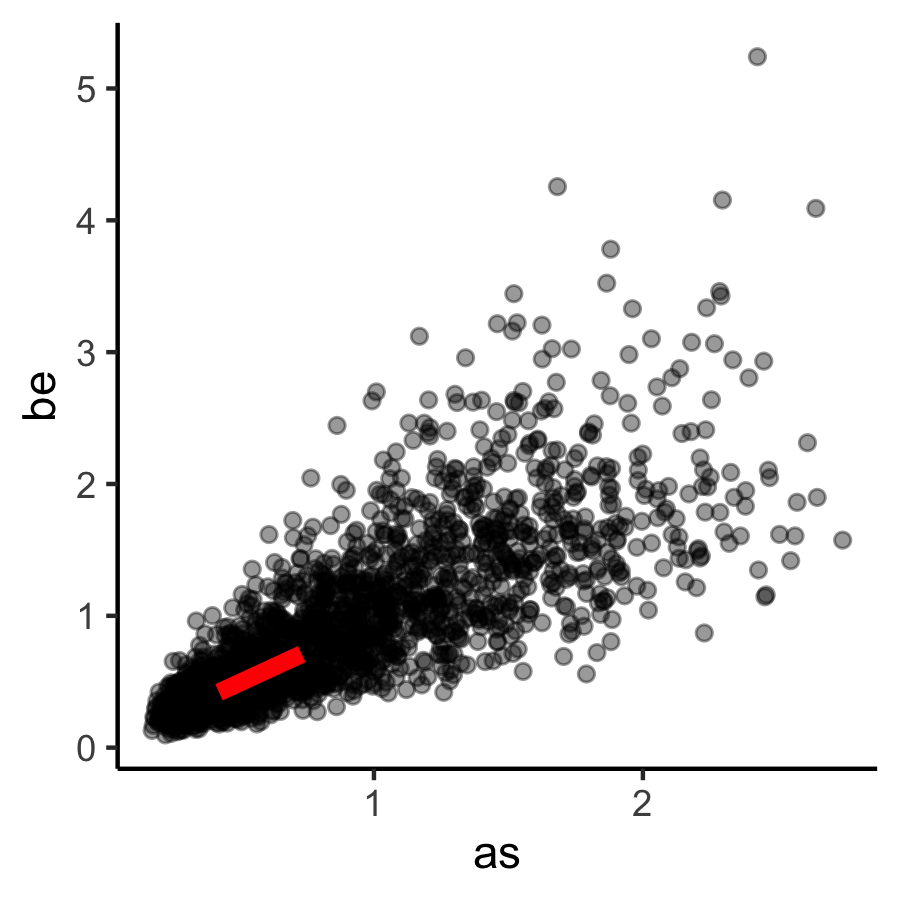
\includegraphics[height=.8\textheight]{../analyses/output/as_be_scatter_j2.png} $$E(y^{a+2, b+2}) - E(y^{a+1,b+1})$$}%
    		 \only<5>{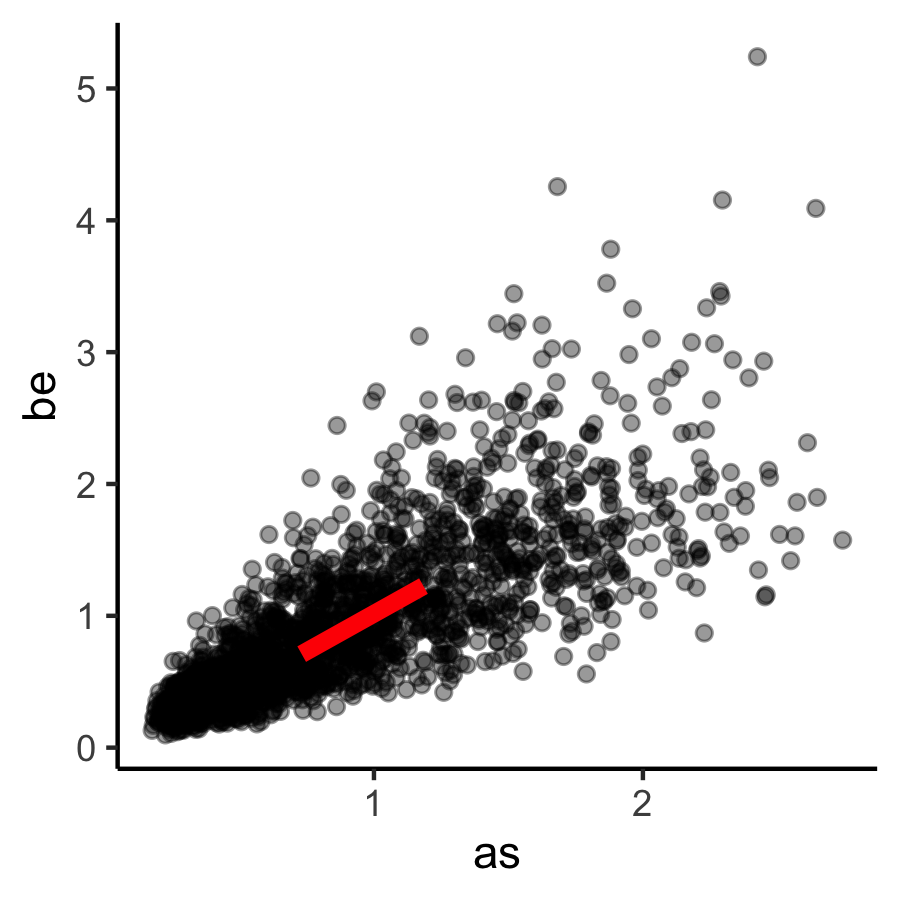
\includegraphics[height=.8\textheight]{../analyses/output/as_be_scatter_j3.png}$$E(y^{a+3, b+3}) - E(y^{a+2,b+2})$$}%
    		 \only<6>{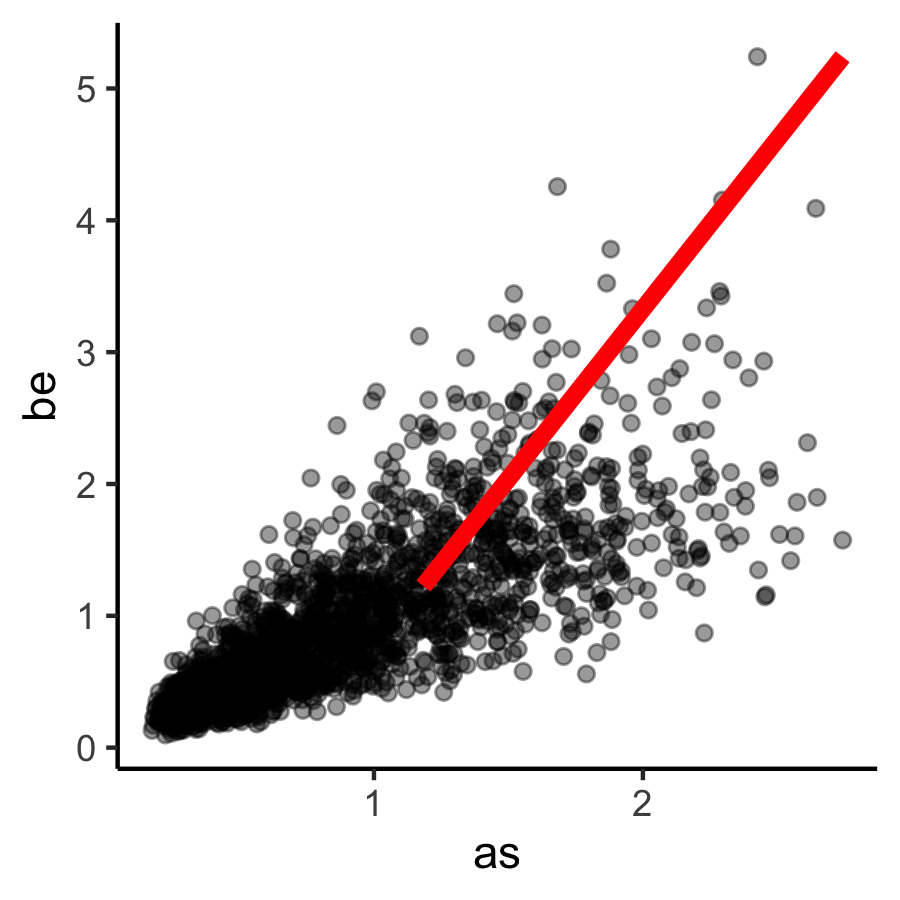
\includegraphics[height=.8\textheight]{../analyses/output/as_be_scatter_j4.png}$$E(y^{a+4, b+4}) - E(y^{a+3,b+3})$$}%
    \end{column}
  \end{columns}
\end{frame}


\begin{frame}[t]{Multiple exposures and marginal structural models}
    	  \begin{columns}
    \begin{column}[c]{.5\textwidth}
      \only<1-2>{
        Estimating a series of effects where we make comparisons of the average MDI at the right and left sides of the red line is roughly equivalent to turning our exposures into indicator variables
      }
      \only<3>{
        Here we see how the average MDI changes as we increase both arsenic and beryllium by one quantile at a time. 
                \bigskip
                
        (note that MDI was not on our scatter plot before)
      }
      \only<4>{
        If causal identification conditions are met (substituting our rough "model" for positivity/sparsity), then this can be interpreted as a regression line for a \textbf{marginal structural model}, which is just a model for average potential outcomes $E(y^{a,b}$)

      }
      \only<5->{
        Methods like Bayesian kernel machine regression\footnotemark{} and quantile g-computation\footnotemark{} \emph{can} give estimates from a \textbf{marginal structural model}. Quantile g-computation actually fits a model where we assume a parametric marginal structural model, giving a smooth regression line, possibly with a polynomial curve.

      }
    \end{column}
    \begin{column}[c]{.5\textwidth}
        		 \only<1>{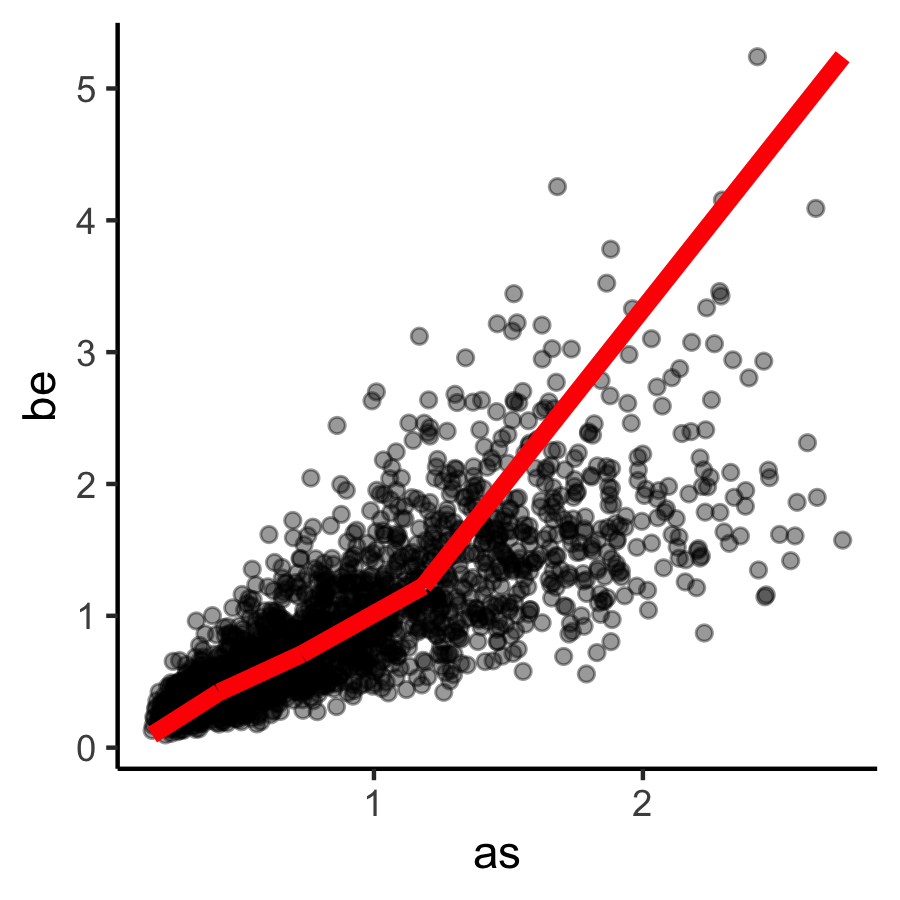
\includegraphics[height=.8\textheight]{../analyses/output/as_be_scatter_j5.png}}%
        		 \only<2-4>{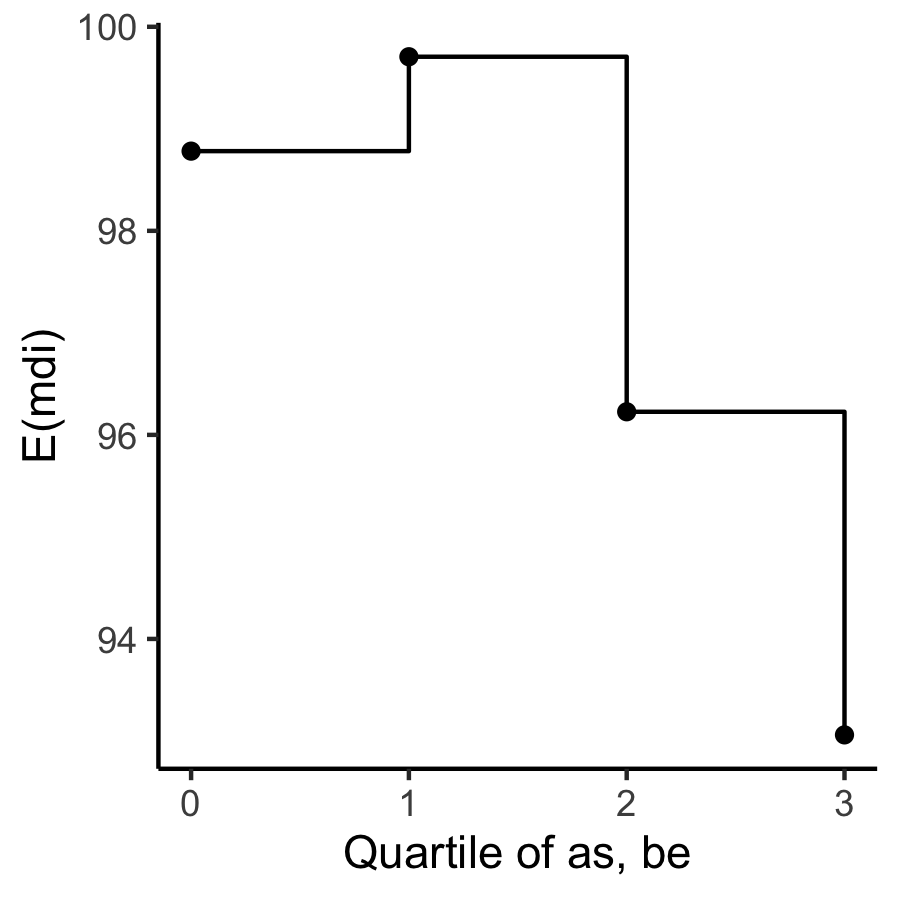
\includegraphics[height=.8\textheight]{../analyses/output/as_be_regline_1.png}}%
        		 \only<5>{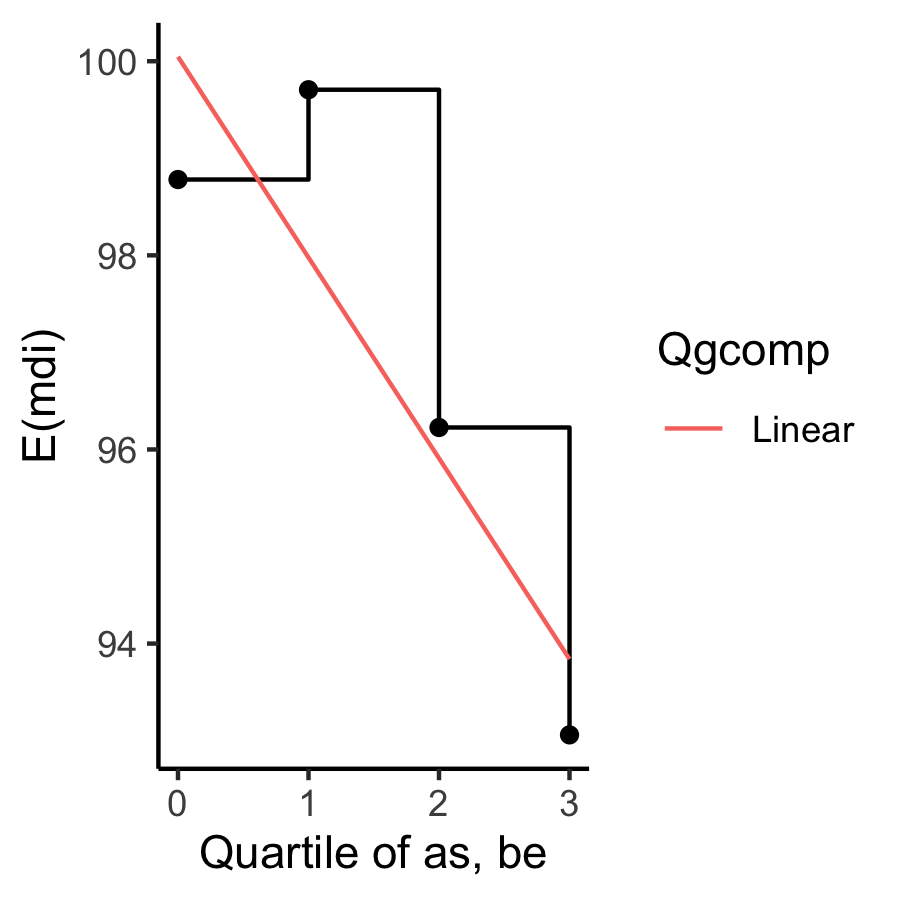
\includegraphics[height=.8\textheight]{../analyses/output/as_be_regline_qgc1.png}}%
        		 \only<6>{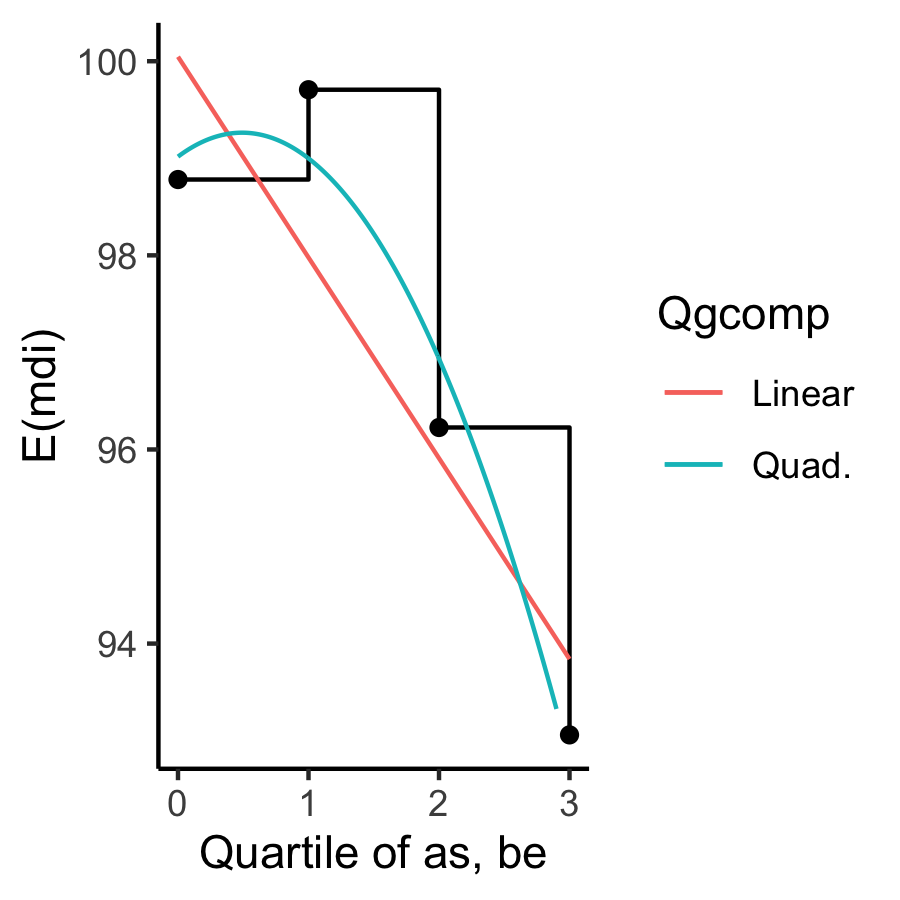
\includegraphics[height=.8\textheight]{../analyses/output/as_be_regline_qgc2.png}}%
    \end{column}
  \end{columns}

      \only<5->{
      \footnotetext[15]{\tiny Bobb, Jennifer F., et al. (2015) Bayesian kernel machine regression for estimating the health effects of multi-pollutant mixtures. Biostatistics 16(3), 493-508.}
      \footnotetext{\tiny Keil, A. P. et al (2020). A quantile-based g-computation approach to addressing the effects of exposure mixtures. Environmental health perspectives, 128(4), 047004.}}
\end{frame}

\begin{frame}[t]{Joint effects and the fundamental problem of mixtures}
  \begin{columns}
    \begin{column}[c]{.5\textwidth}
    One consequence of the fundamental problem of mixtures is that estimates of independent effects of a given exposure (here $\beta_1$) lose precision as correlation $\uparrow$
    \bigskip
    
    In contrast, marginal structural parameters for the joint effects of multiple exposures (here $\psi$) can \emph{gain} precision\footnotemark
     \bigskip
    
   Estimating joint effects may sometimes be a more efficient use of data than estimating independent effects in search of bad actors 
    \end{column}
    \begin{column}[c]{.5\textwidth}
    \begin{figure}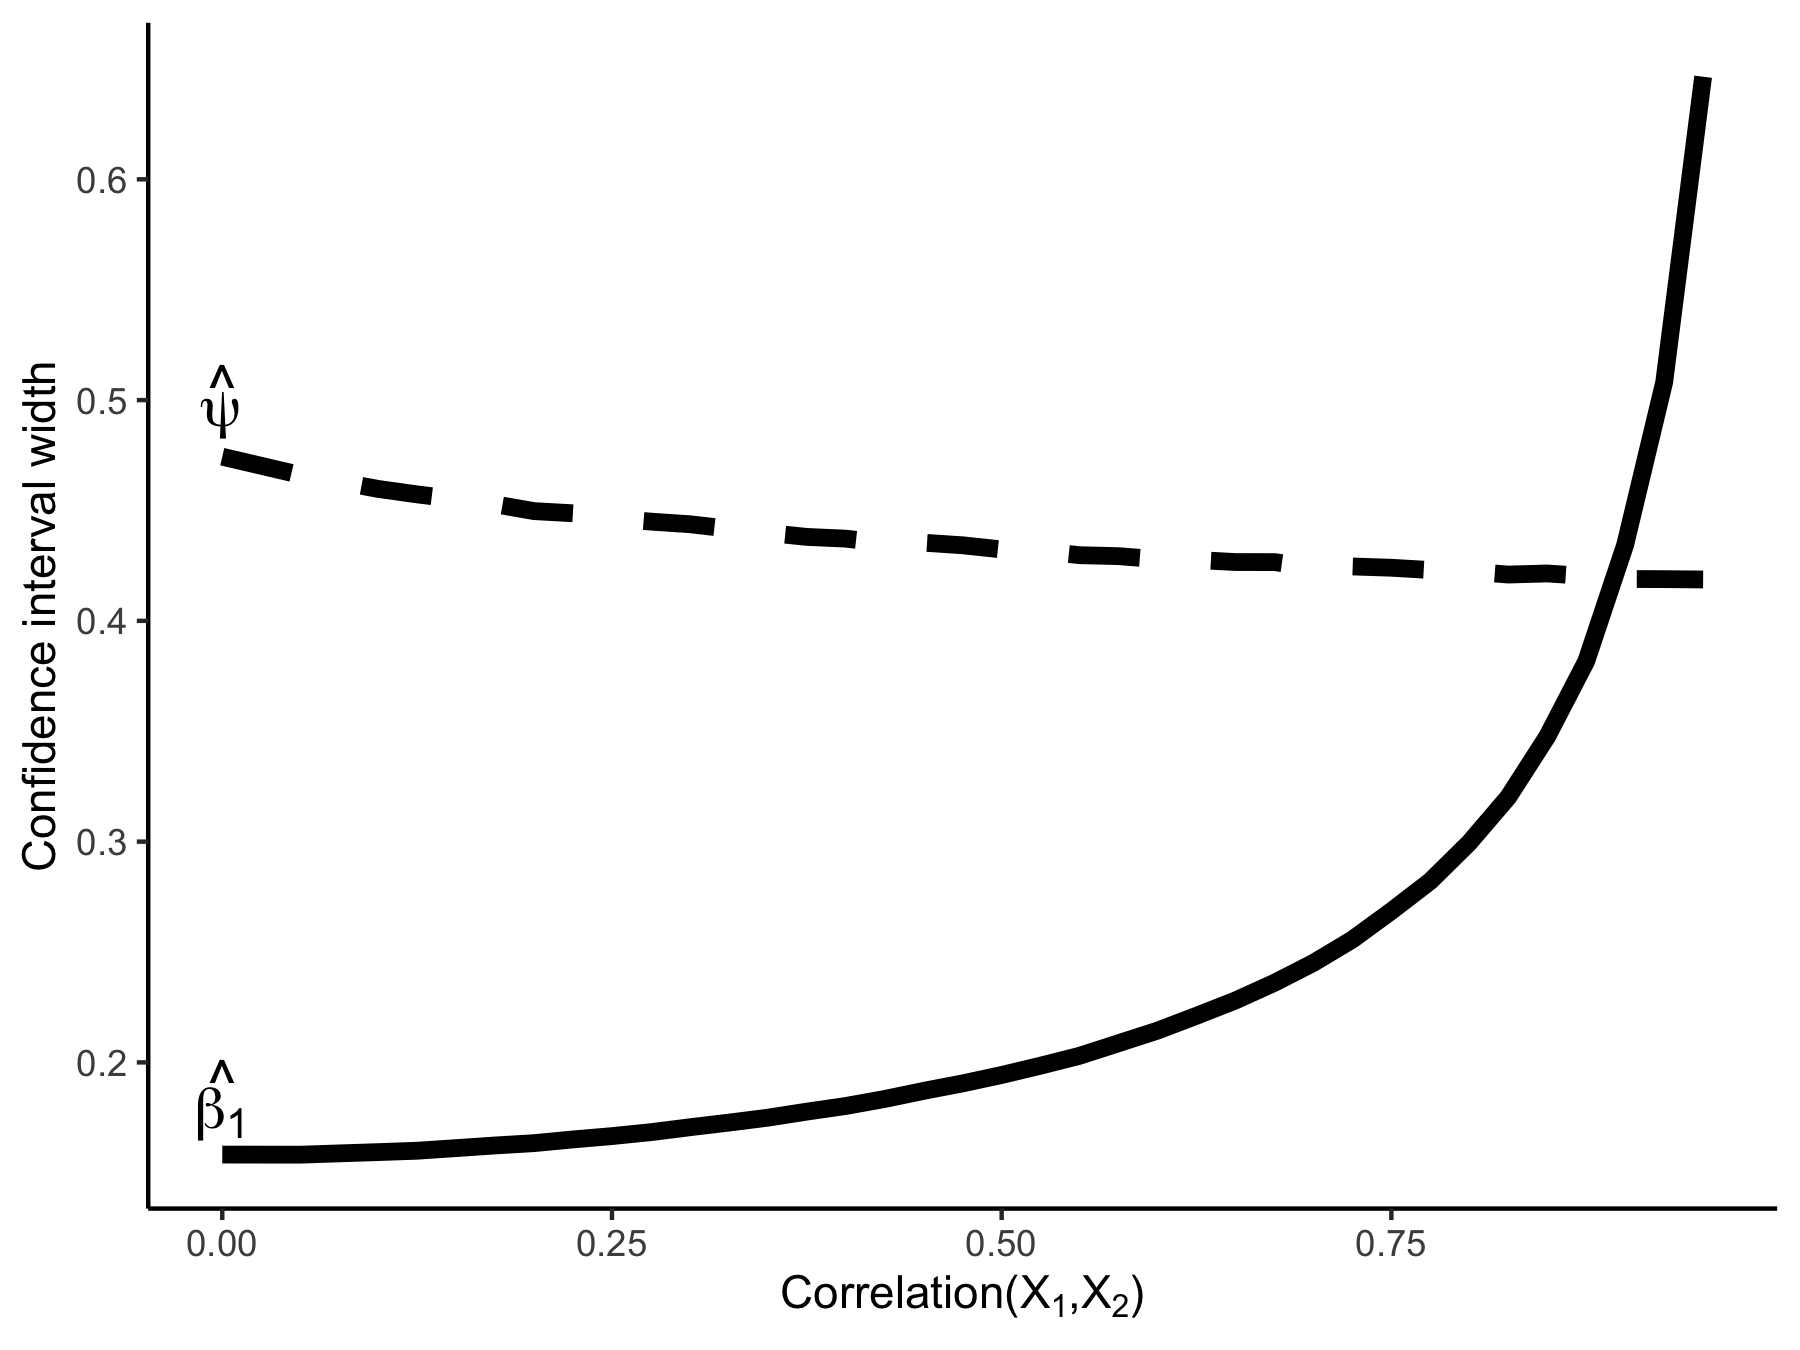
\includegraphics[width=\textwidth]{img/afig1_rev1.png}\end{figure}
    \end{column}
  \end{columns}
\footnotetext{\tiny Keil, A. P. et al (2020). A quantile-based g-computation approach to addressing the effects of exposure mixtures. Environmental health perspectives, 128(4), 047004.}



\end{frame}


%%%%%%%%%%%%%%%%
%\begin{frame}[t]{Textbook examples and continuous exposures}
%	\only<1>{
%	Recall how we represented potential outcomes with 2 new data colums for binary exposures:
%			\begin{center}
%			\begin{tabular}{lccccccc}\hline
%				id & W   & A   & Y   & Y$^{yes}$ & Y$^{no}$ \\\hline
%				1  & 2.9 & yes & no  & no         & ?        \\
%				2  & 0.5 & no  & yes & ?         & yes        \\
%				\hline
%			\end{tabular}
%		\end{center}
%	}
%	%
%	\only<2>{
%	Now consider a continuous exposure (e.g.A= $\mu$g/m$^3$ of airborne arsenic) that could take on many possible values
%	\begin{center}
%		\begin{tabular}{lccccccc}\hline
%			id & W   & A   & Y   & Y$^{-\infty}$         & Y$^{\infty}$           \\\hline
%			1  & 2.9 & 0.30 & no  & ? & ?                  \\
%			2  & 0.5 & 0.87  & yes & ?                 & ? \\
%			\hline
%		\end{tabular}
%	\end{center}
%	}
%	%
%	\only<3>{
%	We can again fill in some outcomes
%	\begin{center}
%		\begin{tabular}{lccccccc}\hline
%			id & W   & A  & Y   & Y$^{0.30}$         & Y$^{0.87}$           \\\hline
%			1  & 2.9 & 0.30 & no  & no & ?                  \\
%			2  & 0.5 & 0.87  & yes & ?                 & yes \\
%			\hline
%		\end{tabular}
%	\end{center}
%	}
%	%
%	\only<4>{
%	But what about other possible values of exposure?
%	\begin{center}
%		\begin{tabular}{lccccccccc}\hline
%			id & W   & A  & Y   & Y$^{0.30}$         & Y$^{0.87}$  & Y$^{1.0}$ & Y$^{3.1}$           \\\hline
%			1  & 2.9 & 0.30 & no  & no & ?& ?& ?                  \\
%			2  & 0.5 & 0.87  & yes & ?                 & yes & ?& ?\\
%			\hline
%		\end{tabular}
%	\end{center}
%	}
%	\only<5->{
%	But what about other possible values of exposure?
%	\begin{center}
%		\begin{tabular}{lcccccccccc}\hline
%			id & W   & A  & Y   & Y$^{0.0}$ & \ldots & Y$^{0.30}$  & \ldots & Y$^{0.87}$& \ldots   & Y$^{\infty}$           \\\hline
%			1  & 2.9 & 0.30 & no  & ?& \ldots& no &\ldots& ?&\ldots& ?                  \\
%			2  & 0.5 & 0.87  & yes & ?& \ldots& ?&\ldots                 & yes & \ldots& ?\\
%			\hline
%		\end{tabular}
%	\end{center}
%		\bigskip
%		
%		\visible<6>{
%		With binary exposures, we typically observe lots of individuals with $A=1$ and $A=0$ in the observed data, so we have some hope that the sparsity is not an issue (e.g. estimated $Pr(A=a) > 0$ at all levels of confounders, akin to positivity) and we can \emph{estimate} a causal effect.
%		\bigskip
%		
%		For continuous exposures, sparsity is guaranteed so the usual tools just do not seem to apply to these settings.
%		}
%	}
%
%\end{frame}